%=============================================================================
%
% MULTIMAT 2017 Suggested Abstract Template
%
% !!!!!!!!!!!!!!!!!!!!!!!!!!!!!!!!!!!!!!!!!!!!!!!!!!!!!!!!!!!!!!!!!!!!!!!!!!!
% !!!!!!!!! ALL SUBMISSIONS MUST BE LIMITED TO 1 PAGE, NO EXCEPTIONS !!!!!!!!
% !!!!!!!!!    ALL SUBMISSIONS MUST BE IN PDF FORMAT, NO EXCEPTIONS  !!!!!!!!
% !!!!!!!!!!!!!!!!!!!!!!!!!!!!!!!!!!!!!!!!!!!!!!!!!!!!!!!!!!!!!!!!!!!!!!!!!!!
%=============================================================================

%=============================================================================
%                           Formatting Options
%=============================================================================

\documentclass[11pt,a4paper]{article}
\usepackage{exscale,times}
\usepackage{graphicx}

\setlength{\parindent}{0pt}
\setlength{\parskip}{5pt plus 2pt minus 1 pt}
\topmargin  -5mm
\evensidemargin 8mm
\oddsidemargin  2mm
\textwidth  158mm
\textheight 230mm
\frenchspacing
\sloppy

%=============================================================================
%                        (Possibly) Useful Commands
%=============================================================================

\newcommand{\refEq}[1]{(\ref{eq:#1})}
\newcommand{\refChap}[1]{Chapter \ref{chap:#1}}
\newcommand{\refFig}[1]{Figure \ref{fig:#1}}
\newcommand{\refSec}[1]{Section \ref{sec:#1}}
\newcommand{\refTab}[1]{Table \ref{tab:#1}}
\newcommand{\refApp}[1]{Appendix \ref{app:#1}}
\newcommand{\newEq}[2]{\begin{equation} \label{eq:#1} #2 \end{equation}}

%=============================================================================
%                       Declarations for Front Matter
%=============================================================================

\begin{document}

\pagestyle{empty}

\begin{center}
%
% <<< INSERT TITLE HERE >>> 
%
{\fontsize{14}{20}\bf \textit{Serious Numerics for Serious Physics}:
  Nonlocal Transport Hydrodynamic Model on Curvilinear Meshes}
%{\fontsize{14}{20}\bf Serious Numerics for Serious Physics:
%  Nonlocal Transport Hydrodynamic Model on Curvilinear Meshes}
\end{center}

%
% <<< INSERT AUTHORS HERE >>> 
%
\begin{center}
%\textbf{M. Holec$^\dagger$}\\
\textbf{Milan Holec}\\
%
% <<< INSERT AFFILIATIONS HERE >>> 
%
%$^\dagger${
%             %First Department, First Institution 
%             Universit\'{e} de Bordeaux - CNRS - CEA, CELIA, UMR 5107, 
%			 F-33405 Talence, France
%			 ({\tt milan.holec@u-bordeaux.fr}) 
%          }                   
\end{center}
%
% <<< INSERT KEYWORDS HERE >>>
%
{\bf Keywords}: 
  nonlocal transport; 
  high-order methods; 
  %finite element method; 
  %Lagrangian methods;
  multi-material hydrodynamics;
  curvilinear meshes.

\begin{center}
\textbf{ABSTRACT}\\[1mm]
\end{center}
%
% <<< INSERT ABSTRACT TEXT HERE >>>
%
A~novel high-order method for solving the~Bhatnagar-Gross-Krook form of 
the~Boltzmann transport equation is presented \cite{DGBGKT}.  
Consequently, the~classical diffusive transport closure to the~Euler equations 
in a~moving Lagrangian frame can be generalized to the~nonlocal regime. 
Our approach presents a~phase-space (including photon and electron momentum) 
extension of the~general high-order curvilinear finite element approach 
for solving Lagrangian hydrodynamics \cite{LAGHOS}. 
%The~numerical approximation of the~transport equation implemented
%directly within the~model of compressible hydrodynamics brings 
%new possibilities of using the~fluid codes under extreme conditions when 
%the~traditional diffusion transport is no more valid. In many applications 
%as astrophysics or inertial confinement fusion, the~generated plasma very 
%often takes place under nonlocal transport conditions. 
We discretize the~transported quantity in space and momentum using 
a~discontinuous Galerkin high-order basis of arbitrary polynomial degree 
defined on a~curvilinear mesh via a~corresponding high-order parametric 
mapping from a~standard reference element. Even though extra dimensions of 
momentum need to be discretized, the~computational cost remains comparable 
with usual diffusion transport methods. 
By the~means of hydrodynamic simulations, the~effect of nonlocal transport is 
investigated for high-power laser interactions with matter \cite{PETE}. 
%Subsequently, 
%the~obtained plasma profiles manifestly demonstrate that the~classical 
%diffusive electron transport cannot model properly the~physics of ablation. 
%and that the~Hugoniot jump condition determining the shock velocity can be 
%significantly altered due to the~nonlocal transport preheat. 
%The obtained results stress the~importance and applicability of our nonlocal 
%transport scheme.
%
% <<< FIGURES ARE OPTIONAL >>>
%
\begin{figure}[htbp]
\centering
  %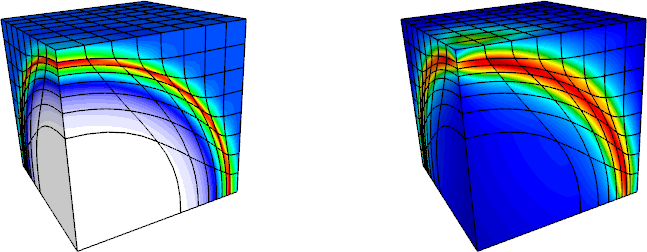
\includegraphics[height=2in]{figs_NTH/nth_sedov.png} \\
  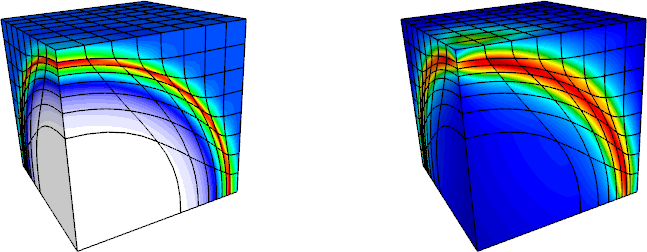
\includegraphics[height=0.3\textwidth]{figs_NTH/nth_sedov.png}
  \begin{tabular}{cc}
    LAGHOS $\qquad\qquad\qquad\qquad\qquad\qquad\qquad$ & NTH
  \end{tabular} 
  \caption{Left: LAGHOS - curvilinear mesh of Sedov problem. 
           Right: Nonlocal Transport Hydrodynamics (NTH) - 
		   high-order radiation energy density computed on the~curvilinear mesh.
  \label{fig:FirstFigure}}
\end{figure}

%
% <<< REFERENCES ARE OPTIONAL >>>
%

\begin{thebibliography}{10}

\bibitem{DGBGKT} M. Holec, J. Limpouch, R. Liska and S. Weber,
``High-order discontinuous Galerkin nonlocal transport and energy equations 
scheme for radiation hydrodynamics'',
\textit{International Journal for Numerical Methods in Fluids}, 83, pp.~779, 2017.
\bibitem{LAGHOS} V. Dobrev, Tz. Kolev and R. Rieben,
``High-order curvilinear finite element methods for Lagrangian
hydrodynamics'',
\textit{SIAM J. Sci. Comp.}, 34, pp.~B606--B641 , 2012.
\bibitem{PETE} K. Falk, M. Holec, C. J. Fontes, C. L. Fryer, C. W. Greeff, 
H. M. Johns, D. S. Montgomery, D. W. Schmidt and M. Smid,
``Measurement of preheat due to nonlocal electron transport in warm dense 
matter'',
\textit{Physical Review Letters}, In press.
\end{thebibliography}

%
% <<< INSERT OPTIONAL ACKNOWLEDGMENTS  >>>
%
%This work performed under the auspices of \ldots

\end{document}
